\documentclass[12pt,a4paper,fleqn]{article}
\title{Progress Report}
\author{Syed Ahmad Raza}
\date{2016.12.22}
\usepackage{mathtools}
\usepackage{graphicx}
\usepackage{color}          % for color eps output
%\usepackage{layouts}       % for: \printinunitsof{in}\prntlen{\textwidth}

\begin{document}
\maketitle
\section*{Derivation of central difference formula for\newline second
derivative}

We know that
\begin{equation}
f_{i+1} = f_i + \left.\frac{df}{dx}\right|_i(x_{i+1} - x_i) +
\left.\frac{d^2f}{dx^2}\right|_i\frac{(x_{i+1} - x_i)^2}{2!} + \ldots
\end{equation}
\begin{equation}
f_{i-1} = f_i + \left.\frac{df}{dx}\right|_i(x_{i-1} - x_i) +
\left.\frac{d^2f}{dx^2}\right|_i\frac{(x_{i-1} - x_i)^2}{2!} + \ldots
\end{equation}

Adding equations (1) and (2) and neglecting the higher order terms,
\begin{equation}
\begin{split}
f_{i+1} + f_{i-1} = \quad &2f_i + \left.\frac{df}{dx}\right|_i(x_{i+1} - x_i +
x_{i-1} - x_i)
\\& + \left.\frac{d^2f}{dx^2}\right|_i\frac{(x_{i+1} - x_i)^2}{2} +
\left.\frac{d^2f}{dx^2}\right|_i\frac{(x_{i-1} - x_i)^2}{2}
\end{split}
\end{equation}

For \emph{equally spaced intervals},
\begin{equation*}
x_{i+1} - x_i = x_i - x_{i-1} = \Delta x
\end{equation*}
\begin{equation*}
x_{i+1} - x_i + x_{i-1} - x_i = 0 
\end{equation*}

Substituting in equation (3), we get
\begin{equation*}
f_{i+1} + f_{i-1} = 2f_i + 2\left.\frac{d^2f}{dx^2}\right|_i\frac{(\Delta
x)^2}{2}
\end{equation*}
\begin{equation}
\left.\frac{d^2f}{dx^2}\right|_i = \frac{f_{i+1} - 2f_i + f_{i-1}}{(\Delta
x)^2}
\end{equation}

For \emph{unequally spaced intervals}, from equation (3), we can write
\begin{equation}
\begin{split}
f_{i+1} + f_{i-1} = \quad &2f_i + \left.\frac{df}{dx}\right|_i(x_{i+1} - x_i +
x_{i-1} - x_i)
\\& + \left.\frac{d^2f}{dx^2}\right|_i\left[\frac{(x_{i+1} - x_i)^2 + (x_{i-1} -
x_i)^2}{2}\right]
\end{split}
\end{equation}

We also know that the central difference formula for the first derivative,
neglecting the higher order terms, may be written as
\begin{equation}
\left.\frac{df}{dx}\right|_i = \frac{f_{i+1} - f_{i-1}}{x_{i+1} - x_{i-1}}
\end{equation}

Substituting equation (6) in equation (5), we have
\begin{equation*}
\begin{split}
f_{i+1} + f_{i-1} = \quad &2f_i + \frac{f_{i+1} - f_{i-1}}{x_{i+1} -
x_{i-1}}(x_{i+1} - 2x_i + x_{i-1})
\\& + \left.\frac{d^2f}{dx^2}\right|_i\left[\frac{(x_{i+1} - x_i)^2 + (x_{i-1} -
x_i)^2}{2}\right]
\end{split}
\end{equation*}

Rearranging this equation,
\begin{equation*}
\left.\frac{d^2f}{dx^2}\right|_i = \quad \frac{(f_{i+1} + f_{i-1}) - 2f_i -
(f_{i+1} - f_{i-1})\dfrac{(x_{i+1} - 2x_i + x_{i-1})}{x_{i+1} -
x_{i-1}}}{\dfrac{(x_{i+1} - x_i)^2 + (x_{i-1} - x_i)^2}{2}}
\end{equation*}
\begin{equation}
\begin{split}
\left.\frac{d^2f}{dx^2}\right|_i = \quad &\frac{2(f_{i+1} + f_{i-1})}{(x_{i+1} -
x_i)^2 + (x_{i-1} - x_i)^2}
\\& - \frac{4f_i}{(x_{i+1} - x_i)^2 + (x_{i-1} -
x_i)^2}
\\& - \frac{2(f_{i+1} - f_{i-1})(x_{i+1} - 2x_i + x_{i-1})}{(x_{i+1} -
x_{i-1})[(x_{i+1} - x_i)^2 + (x_{i-1} - x_i)^2]}
\end{split}
\end{equation}

For the case of of equally spaced data with $x_{i+1} - x_i = x_i -
x_{i-1} = \Delta x$, this again reduces to equation (4).

\newpage
\section*{Numerical solution for 2D heat transfer}
A C++ code was written to solve a simple problem of 2D heat transfer in a block
of pure silver (99.9\%).

Initial condition was $T_i=25^{\circ}C$.

Boundary conditions were selected as follows:
\begin{enumerate}
\item $T_{xi}=25^{\circ}C$ at $x=0$
\item $T_{xf}=25^{\circ}C$ at $x=L$
\item $T_{yi}=25^{\circ}C$ at $y=0$
\item $T_{yf}=50^{\circ}C$ at $y=L$
\end{enumerate}

The analytical solution to this problem is given by:
\begin{equation}
T(x, y) =
\frac{2T_3}{\pi}\sum\limits_{n=1}^{\infty}\left[\frac{(-1)^{n+1}+1}{n}\right]
\frac{\sin\lambda_nx\sinh\lambda_ny}{\sinh\lambda_nW} + T_1\end{equation}
where
\begin{equation}
T_1 = T_{xi} = T_{xf} = T_{yi}
\end{equation}
and
\begin{equation}
T_3 = T_{yf} - T_1
\end{equation}

Forward in time center in space (FTCS) method was used with the following
formula:
\begin{equation}
T_i^{n+1} = T_i^n + \Delta t \alpha(\frac{\partial^2T}{\partial x^2} +
\frac{\partial^2T}{\partial y^2})
\end{equation}

A time step of 0.001 was utilized with $200\times200$ grid intervals in both x
and y directions. %Two sets of boundary conditions were considered.

\begin{figure}[p!]
\centering
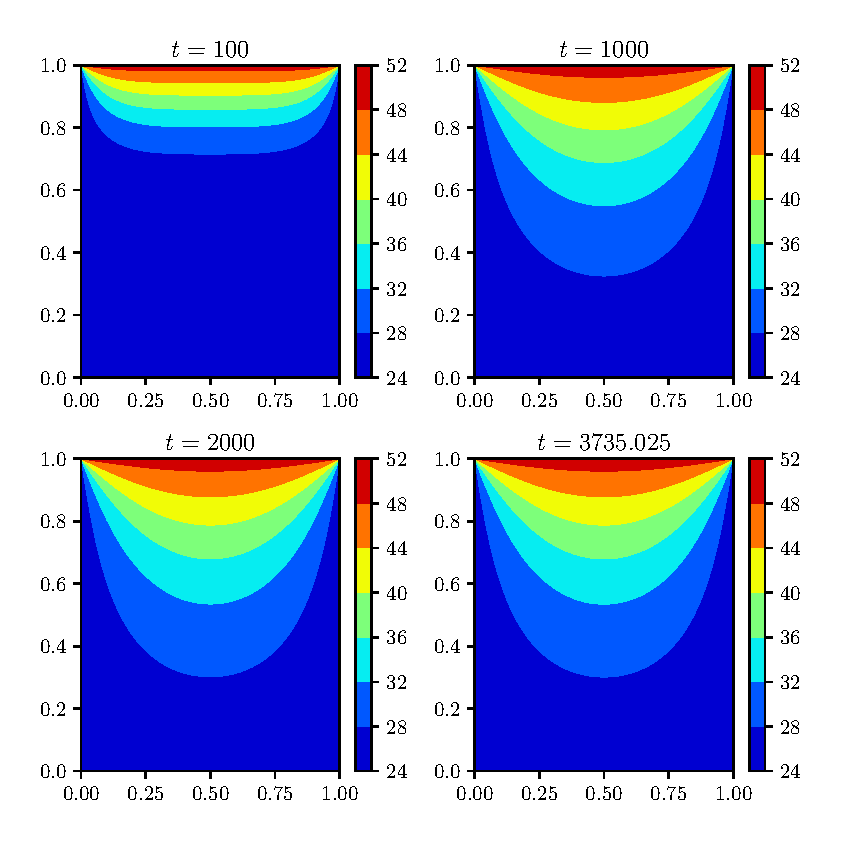
\includegraphics[width=\linewidth]{ht2dCase01.eps}
\caption{Plots for various values of time (time step of 0.001).}
\end{figure}

% \newpage
% Boundary conditions for the second case were selected as follows:
% \begin{enumerate}
% \item $T_{xi}=25^{\circ}C$ at $x=0$
% \item $T_{xf}=50^{\circ}C$ at $x=L$
% \item $T_{yi}=25^{\circ}C$ at $y=0$
% \item $T_{yf}=50^{\circ}C$ at $y=L$
% \end{enumerate}
% The initial condition was kept the same. However, steady state was not achieved
% for the test durations used.
% 
% \begin{figure}[p!]
% \centering
% 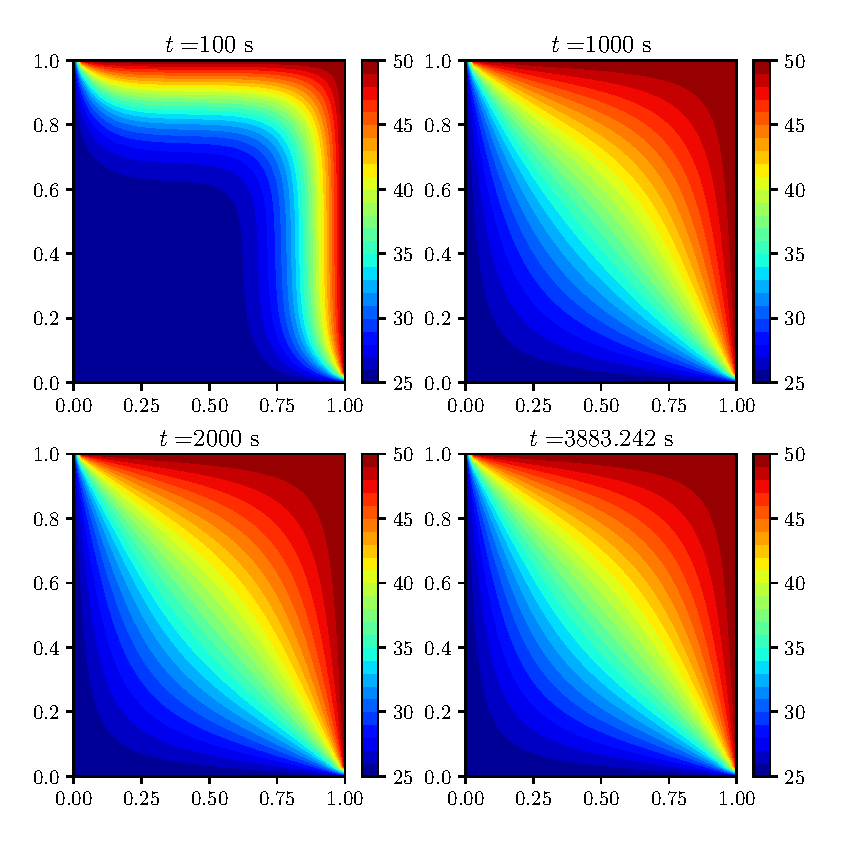
\includegraphics[width=\linewidth]{ht2dCase02.eps}
% \caption{Plots for the first case with various values of time (time step of
% 0.001).}
% \end{figure}
\end{document}